\documentclass[12]{article}
\usepackage{fullpage}
\usepackage{graphicx}
\usepackage[utf8]{inputenc}
\usepackage{amsmath}
\usepackage{graphics}
\usepackage{float}
\usepackage{xcolor}
\usepackage{geometry}
\usepackage{tikz}
\usetikzlibrary{shapes, arrows}
\usepackage[utf8]{inputenc}
\usepackage{amsmath}
\usepackage{graphics}
\usepackage{xcolor}
\usepackage{enumitem}
\usepackage{array}


\begin{document}

\section*{CHAPTER 3}
\section*{FACTOR ANALYSIS}
	\subsection{Conceptual model Factor Analysis}
	\subsubsection{Introduction}
Factor analysis describes, if possible, the covariance 
relationships among many variables in terms of a few underlying, but   unobservable, random quantities called factors. \\
The general model of FA assumes that the observed variables are linear combinations of a smaller number of latent factors, which are unobserved variables that are assumed to be the true causes of the observed variables.\\
Additionally, factor model is motivated by the following argument: Suppose variables can be grouped by their correlations. That is, suppose all variables within a particular group are highly correlated among themselves, but have relatively small correlations with variables in a different group. Then it is conceivable that each group of variables represents a single underlying construct, or factor, that is responsible for the observed correlations. \\

\subsubsection{Difference between Principal Components Analysis and Factor Analysis}
\begin{enumerate}[label=\roman*]
	\item Principal components are linear combinations of the original variables while in FA original variables are expressed as linear combination of the factors.
	\item In PCA, we account for large part of of the total variation of the variables while FA we account for contrivances or correlations among variables.
\end{enumerate}
\subsubsection{The Orthogonal Factor Model}
Let $X$ be an observable random vector, with $p$ components, mean $\mu$ and covariance matrix $\Sigma$. \\
The factor model postulates that $X$ is linearly dependent upon a few unobservable random variables $F_1, F_2, F_3, \cdots, F_m$, called \emph{common factors}, and $p$ additional sources of variations $\epsilon_1, \epsilon_2, ..........\epsilon_p$ called \emph{Errors/ residual}.\\

\noindent The general model of a factor analysis is(Johnson \& Wichern, 2007):
	\begin{equation}
	X_1- \mu_1=\beta_1 F + \epsilon_1
\end{equation}
\noindent For a $m$ common factor(s) is;
	\[
	\left(
	\begin{matrix}
		x_1 - \mu_1= \beta_{11}F_1 +...+\beta_{1m}F_m +\epsilon_1 \\
		x_2 - \mu_2= \beta_{21}F_1 +...+\beta_{2m}F_m +\epsilon_2 \\
		x_3 - \mu_3 = \beta_{31}F_1+...+\beta_{3m}F_m +\epsilon_3 \\
		.                  .              .      \\
		.                  .               .     \\
		.                  .              .     \\
		x_p - \mu_p =\beta_{p1}F_1+...+\beta_{pm}\eta_m +\epsilon_p \\                
		
	\end{matrix}
	\right)
	\]
\noindent Where:
\begin{enumerate}[label=\roman*]
\item $\mu_i$ is mean of variable $i$\\
\item $\beta_{ij}$ is $(p\times m)$ factor loading of the $i^{th}$ variable on the $j^{th}$ factor. \\
\item $\epsilon_i$ is $(p \times 1)$ the error associated with $i^{th}$ response $X_i$.\\
\item $F_j$ refers to the $m \times1$ of the latent(unobservable) variables\\

\end{enumerate}

\noindent The matrix notation 
\begin{equation}
	\left(
	\begin{matrix}
		x_1\\
		x_2\\
		\vdots \\
		x_p\\
	\end{matrix}
	\right) - \left(
	\begin{matrix}
		\mu_1\\
		\mu_2\\
		\vdots \\
		\mu_p\\
	\end{matrix}
	\right) = 
	\left(\begin{matrix}
		\beta_{11} & .&.&.& \beta_{1m}\\
		\beta_{21} &  .&.&. & \beta_{2m}\\
		\vdots\\
		\beta_{p1}  & .&.&. &\beta_{pm}\\
	\end{matrix}\right) \times
	\left(\begin{matrix}
		F_1\\
		F_2\\
		\vdots\\
		F_m\\
	\end{matrix}\right)+ \left(\begin{matrix}
		\epsilon_1\\
		\epsilon_2\\
		\vdots\\
		\epsilon_p\\
	\end{matrix}\right)
\end{equation}

\begin{equation}
X- \mu= L F + \epsilon
\end{equation}

\noindent Where:\\
$\mu$ is mean of variable $i$\\
\noindent $L$ is the matrix of factor loadings\\
\noindent $F$ refers to the matrix of the latent(unobservable) variables\\
\noindent $\epsilon$ is the matrix of the residuals

\subsubsection*{Assumptions of the the FA model}
\begin{enumerate}[label=\roman*]
\item $E(F) = 0$
\item $E(\epsilon) = 0$
\item $Cov(\epsilon)= \Psi $ where $\Psi$ is a diagonal matrix

 $$\begin{pmatrix}
	\psi_{1} & 0 & \cdots & 0 \\
	0 & \psi_{2} & \cdots & 0 \\
	\vdots & \vdots & \ddots & \vdots \\
	0 & 0 & \cdots & \psi_{p}
\end{pmatrix}$$
\item $F$ and $\epsilon$ is independent.
\end{enumerate}
\subsubsection{Covariance Structure for the Orthogonal Factor Model}
From equation (3) above, the orthogonal factor model implies a covariance structure for X.
\begin{align*}
	(X-\mu)(X-\mu)' &= (LF+\epsilon)(LF+\epsilon)' \\
	&= (LF+\epsilon)((LF)'+\epsilon') \\
	&= LF(LF)' + \epsilon(LF)' + LF\epsilon' + \epsilon\epsilon \\
\end{align*}
Therefore;\\
\begin{align*}
	\Sigma & = Cov(X) = E(X-\mu)(X-\mu)' \\
	&=LE(FF')L' + E(\epsilon F')L' + LE(F\epsilon')+E(\epsilon\epsilon')\\
	&= LL' + \Psi
\end{align*}
similarly;
$$Cov(X,F)= L$$
The model $X-\mu=LF+ \epsilon$ is linear in the common factors.\\
The portion of the variance of the $i^{th}$ variable contributed by the common factors is called \textbf{the $i^{th}$ communality.}\\
The portion of the variance due to the residual factor is reffered to as \textbf{unique variance}.\\
As an illustration consider the equation below,
\begin{equation*}
	\underbrace{\sigma_{ii}}_{Var(X_I)}= \underbrace{\beta_{11}^2 + \beta_{12}^2 + \cdots +\beta_{1m}^2}_\text{Communality} +\underbrace{\psi_i}_\text{Unique variance}
\end{equation*}
Thus,
\begin{align*}
	Var(X_i)= Communality + Unique variance
\end{align*}
\subsection{Estimation of Loadings and Communalities}
Given observations $x1 , x2, ... ,Xn$ on $p$ generally correlated variables, factor analysis seeks to answer the question, Does the factor model, with a small number of factors, adequately represent the data? In essence, we tackle this statistical model~­
building problem by trying to verify the covariance relationship.
\subsubsection{Principal components method}
From a random sample $X_1, X_2, \cdots, X_p$ we obtain the sample covariance matrix $S$ and then we attempt to find an estimator $\hat{L}$ that will approximate the expression $\Sigma=LL' +\Psi$ with $S$ instead of $\Sigma$ i.e
$$S \approx \hat{L}L' + \Psi$$
In Principal factor method we ignore $\Psi$ and factor $S$ into $S=\hat{L}L$; inorder to factor S we use spectoral decomposition $$S=PDP'$$  where;\\
$P$ is the normalized eigenvectors of S as columns

$$D=  \begin{pmatrix}
	\lambda_{1} & 0 & \cdots & 0 \\
	0 & \lambda_{2} & \cdots & 0 \\
	\vdots & \vdots & \ddots & \vdots \\
	0 & 0 & \cdots & \lambda_{p}
\end{pmatrix}$$
$\L$ is estimated as
$$\hat{L}=[\sqrt{\lambda_1}e_1, \sqrt{\lambda_2}e_2, \cdots , \sqrt{\lambda_k}e_k]$$
The $i^{th}$ diagonal element of $\hat{L}L'$ is the sum of squares of the $i^{th}$ row of $\hat{L}$.\\

\noindent The sums of squares of rows and columns of $\hat{L}$ are equal to the communalities and eigenvalues respectively i.e 
$$\hat{h}_i^2 =\sum_{j=1}^{k}\hat{\beta}_{ij}^2$$ which is the sum of square of the $i^{th}$ row of $\hat{L}$.\\
The sum of squares of the $j^{th}$ column of $\hat{L}$ is the $j^{th}$ eigenvalue of $S$ i.e $\lambda_j$\\

\noindent The variance of the $i^{th}$ variable is partitioned into a part due to the factors and due to uniquely to the variable
$$= \hat{h}^2_{i1}+ \hat{h}^2_{i2} + \cdots +\hat{h}^2_{ik} + \Psi_i$$
Thus the $j^{th}$ factor contributes $\hat{h}_{ij}^2$ to $s_{ii}$. The ontribution of the $j^{th}$ factor to the total sample variance $tr(S)=s_{11}+s_{22} +\cdots +s_{pp}$ is therefore; 
$$=\sum_{j=1}^{p}\hat{\beta}_{ij}^2= \hat{\beta}^2_{1j}+ \hat{\beta}^2_{2j}+ \cdots+\hat{\beta}^2_{pj}$$

\noindent Which is the sum of squares of loadings in the coulumn of $\hat{L}$, which is is the same as the $j^{th}$ eigen value.\\
The proportion of the total sample variance due to the $j^{th}$ factor is $$\frac{\lambda_j}{tr(S)}$$ and if the correlation matrix is used, the above proportion is;
$$\frac{\lambda_j}{p}$$
\underline{Note:}\\
There is always some prior expectation concerning the loadings. In particular it is expected that some loadings will be close to zero while others will be negative or positive and substantialy different from zero. For this reason FA usually proceeds in two stages.
\begin{enumerate}
	\item one set of loadings $\beta_{ij}$ is calculated which yields theoritical variances and covariances that fit the observed ones closely as possible according to certain criterion. These loading may however not agree with the prior expectation.
	\item The first loading are rotated in an effort to arrive at another set that fit equally well the observed variances and covariances but are consistent with prior expectation or easily interpreted.
\end{enumerate} 
\newpage
\subsubsection*{Illustration}
\noindent As an illustration, let's consider the below example;\\
\noindent Patients seeking treatment from a certain psychiatry hospital are subjected to three tests on their trends in sleep, happiness and tiredness to tell the severity of their depression. Let Y1, Y2 and Y3 resptively respresent the scores from the 3 tests respectively. The data consists of 5 patients (in a 10 point scale) as below,
\begin{table}[ht]
	\centering
	\begin{tabular}{c c c c}
		
		Patient's Number & Y1 & Y2 & Y3 \\
		
		 1 & 3 & 6 & 5 \\
		
		 2 & 7 & 3 & 3 \\
		 3 & 10 & 9 & 8 \\
		 4 & 3 & 9& 7 \\
		 
		 5 & 10 & 6 & 5 \\
		
	\end{tabular}
		\caption{Patient scores}
		\label{tab:mytable}
\end{table}\\
It is suggested that the scores are functions of two underlying factors(symptoms) F1 and F2 i.e Cognitive symptoms and Affective symptom respectively. Each variable Y is assumed to linearly  related to the two factors

\begin{align*}
	Y1= \mu_1 +\beta_{11}F1 +\beta_{12}F2+ \epsilon_1 \\
	Y2= \mu_2 + \beta_{21}F1 + \beta_{22}F2 + \epsilon_2 \\
	Y3= \mu_3 + \beta_{31}F1+ \beta_{32}F2 + \epsilon_3
\end{align*}
In the measurement of severity of depression,  trend in sleep point patients cognitive symptom  while the level of happiness and tiredness feeling signify the Affective symptoms of depression. The visualization of the loading is represented as;

\begin{figure}[h]
	\centering

		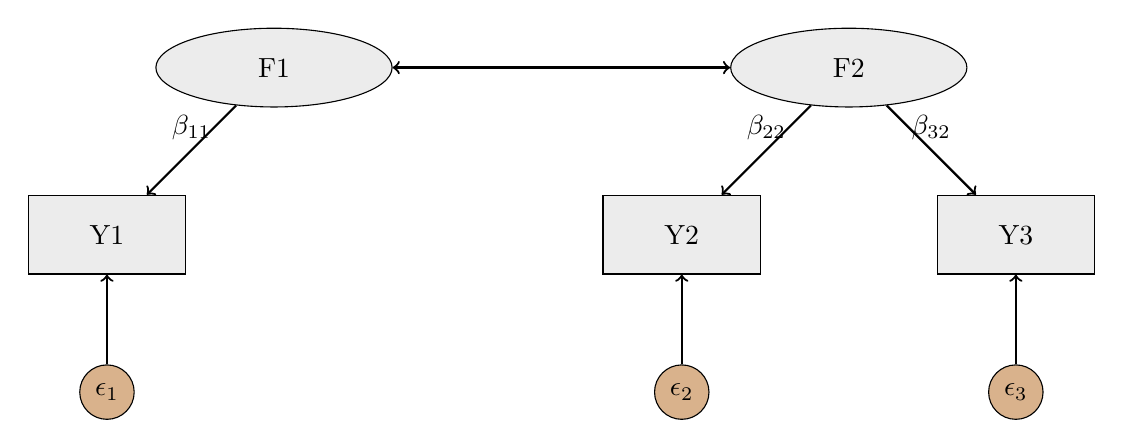
\begin{tikzpicture}[ factor/.style={draw,fill=lightgray!30, ellipse,minimum height=1cm, minimum width=3cm, node distance= {7.3cm}},
			observed/.style={draw, rectangle, minimum width=2cm, minimum height=1cm, fill=lightgray!30,node distance= {3cm}},
			residual/.style={draw,fill=brown!60,  circle, node distance= {2cm}}
			]
			\node [factor](x1) {F1};
			\node [factor](x2)[right of =x1] {F2};
			
			\node [observed](y1) [below left of=x1] {Y1};
			\node [observed](y2) [below left of=x2] {Y2};
			\node [observed](y3) [below right  of=x2] {Y3};
		
			\node [residual](e1) [below of=y1] {$\epsilon_1$};
			\node [residual](e2) [below of=y2] {$\epsilon_2$};
			\node [residual](e3) [below of=y3] {$\epsilon_3$};
			
			
			\draw[thick, black, ->](x1) -- (y1) node[midway, above] {$\beta_{11}$};
			\draw[thick, black, ->] (x2) -- (y2) node[midway, above] {$\beta_{22}$};
			\draw[thick, black, ->] (x2) -- (y3) node[midway, above] {$\beta_{32}$};
			
			\draw[thick, black, ->] (e1) -- (y1);
			\draw[thick, black, ->] (e2) -- (y2);
			\draw[thick, black, ->] (e3) -- (y3);
			
			\draw[thick, black, <->] (x1) -- (x2);
		\end{tikzpicture}
	\caption{Visualization}
	\label{fig:Figure 3.1}
\end{figure}
Thus $Var(Y_i)=\underbrace{\beta^2_{i1} + \beta^2_{i2}}_ \text{Communality} + \underbrace{\psi_i}_\text{specific variance}$\\

\noindent If the factors were perfect predictors of the tests then $\epsilon_1=\epsilon_2=\epsilon_3=0$ and consequently, $\psi_{1}=\psi_{2}=\psi_{3}=0$

$$Cov(Y_i, Y_j)= \beta_{i1}\beta_{j1} + \beta_{i2}\beta_{j2}$$

\noindent Therefore our observed variance- covariance matrix $S$ is;

\begin{table}[ht]
	\centering

	\begin{tabular}{rrrr}
	
		& Y1 & Y2 & Y3 \\ 

		Y1 & 9.84 & -0.36 & 0.44 \\ 
		Y2 & -0.36 & 5.04 & 3.84 \\ 
		Y3 & 0.44 & 3.84 & 3.04 \\ 
	\end{tabular}
\end{table}
\noindent We determine the first set of loadings using principle component method that seeks values of the loadings that bring the the estimates of the total communalities as close as possibe to the total observed variance(Covariance are ignored).\\
From our illustration, the elements of the principal components method are arranged as follows:

\begin{table}[ht]
	\centering

	\begin{tabular}{rrr}
		\hline
		
	Variable & Observed Variance & Communality  \\ 
		
		\\[0.1cm]
		Y1 & $S^2_1$ & $\beta^2_{11}$ + $\beta^2_{12}$ \\ 
		\\[0.2cm]
		Y2 & $S^2_2$ & $\beta^2_{21}$ + $\beta^2_{22}$ \\ 
		\\[0.2cm]
		Y3 & $S^2_3$ & $\beta^2_{31}$ + $\beta^2_{32}$ \\ 
		\\[0.2cm]
		Total& $T_0$ & $T_t$ \\
		\hline
	\end{tabular}
\end{table}
\newpage
\noindent The principal components method determines the values of the $\beta_{ij}$'s which makes the total communality $T_t$ approximate as possible the sum of the observed varianciances, $T_0$.\\
Thus, from our illustration, 
\begin{table}[ht]
	\centering
	
\begin{tabular}{>{\vspace{0.3cm}}ccccc}

		\hline
		
		Variable & Observed Variance &Loadings on ($F_1,\beta_{i1}$)& Loadings on ($F_2,\beta_{i2}$)& Communality  \\ 
		
		\\[0.1cm]
		Sleep Y1 & $9.84$ & 3.136773 &0.023799 &9.98399 \\ 
		\\[0.2cm]
	Happiness	Y2 & $5.04$ &-0.312190 &2.237859 & 5.0255 \\ 
		\\[0.2cm]
	Tiredness	Y3 & $3.04$ & 0.127697 &1.1731884 &3.0157 \\ 
		\\[0.2cm]
		Total& $17.92$ & 9.873125 * &8.007977 *& 17.881 \\
		\hline
	\end{tabular}
	\caption{Solution}
\end{table}\\
\noindent From the solution in the table 2 above, we notice that the solution supports our expectation.\\
\noindent The loadings on $F_1$ are relatively large for $Y1$  but close to zero for $Y2$ and $Y3$; loadings on $F_2$ are close to zero for $Y1$ but relatively high for Y2 and Y3. Implying F1 could be interprated as the cognitive symptom and F2 as Affective symptom.

\end{document}